\chapter{Evaluation and Future Work}
\section{Evaluating Performance}

In order to test the Block Explorer's performance, time measurements were taken for certain actions. First, upon starting the explorer up and letting it fill its database, it was measured how long it took to process a blockchain consisting of more than fifteen thousand blocks. It is important to note, that the majority of the blocks were empty, meaning no transactions were included in them. The miner, the explorer connects to was hosted on an Ubuntu \cite{ubuntu} Virtual Machine, located at the University of Zurich. In Table \ref{tab:load}, the average load times on different machines are presented.

Other measurements that were taken, include the time it took to request and display single items, lists of items and the search function. The results are displayed in Table \ref{tab:query}. In this test, the explorer itself was hosted on an Ubuntu Virtual Machine at the University of Zurich and contained the blockchain with over fifteen thousand blocks. HTML Load Time measured the time it took from the request to the server, until it responded with the HTML file containing the requested blockchain data. Since other files are being loaded, such as style sheets, the time it took to load the entire page is included as well. Testing was conducted using a Computer, connected the University's Network using ethernet and timed using Google Chrome's \cite{chrome} developer tools.

\begin{table}[]
\centering
\caption{Load Times to Copy Fifteen Thousand Blocks From a Miner}
\label{tab:load}
\begin{tabular}{|l|l|l|l|}
\hline
\textbf{Computer} & \textbf{CPU} & \textbf{RAM} & \textbf{Load Time in Minutes} \\ \hline
MacBook Pro & 2.9 GHz Intel Core i5 & 8 GB & 2:17 \\ \hline
Ubuntu VM & 2.4 GHz  Intel Xeon & 2 GB  & 3:29 \\ \hline
\end{tabular}
\end{table}

\begin{table}[]
\centering
\caption{Load Times for Various Requests}
\label{tab:query}
\begin{tabular}{|l|l|l|}
\hline
\textbf{Query}            & \textbf{HTML Load Time} & \textbf{Page Load Time} \\ \hline
Block                     & 25 ms                   & 122 ms                  \\ \hline
Funds Transaction         & 30 ms                   & 121 ms                  \\ \hline
Account with Transactions & 32 ms                   & 119 ms                  \\ \hline
100 Most Recent Blocks    & 63 ms                   & 152 ms                  \\ \hline
Status Page               & 70 ms                   & 744 ms                  \\ \hline
Search of a Block         & 62 ms                   & 151 ms                  \\ \hline
\end{tabular}
\end{table}
\pagebreak

\section{Future Work}
At time of writing, the applications's backend functionality of retrieving blocks from a miner, saving them to the database and returning them upon request is separated from the frontend that displays the returned data. This enables the possibility of switching out the frontend that displays HTML content for a REST API that returns the blockchain data in JSON format. Uses of such an interface could be an integration into the Payment System PWA, which displays data only on request. For example the PWA could display all confirmed transactions for an account in order to make the Payment app more informative, as seen in Figure \ref{fig:pwa_api}.

Another feature, the current block explorer lacks, is frontend optimization for mobile devices. Dynamically styled tables and UI components are needed to accommodate for the many resolutions and aspect ratios of mobile devices. To increase performance, especially on mobile devices, CSS micro-frameworks, such as Furtive \cite{furtive} or Pure.CSS \cite{pure} could be used to keep style sheets at a minimum size. This would also prevent the need for resource-heavy Bootstrap imports and links.
\\
\\
\\

\begin{figure}[h]
  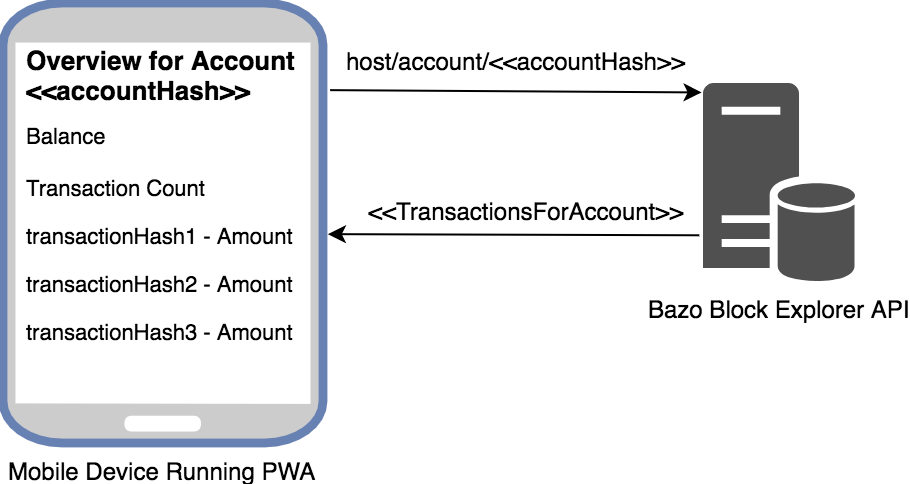
\includegraphics[scale=0.4]{pwa_integration.png}
  \centering
  \caption{Device Running PWA Payment System Requesting a User's Transactions}
  \label{fig:pwa_api}
\end{figure}